\section{El problema de la amistad}

\begin{frame}{El problema de la amistad}
\begin{columns}
\column{0.52\textwidth}
    \begin{block}{Problema}
        En un grupo de 6 personas, ¿siempre existen 3 que se conocen mutuamente o 3 que son mutuamente desconocidos?
    \end{block}
    Modelamos como el grafo completo $K_6$:
    \begin{itemize}
        \item Aristas \textcolor{red}{rojas}: se conocen
        \item Aristas \textcolor{blue}{azules}: desconocidos
    \end{itemize}
    \begin{alertblock}{Pregunta}
        ¿Toda 2-coloración de $K_6$ tiene un triángulo monocromático?
    \end{alertblock}
\column{0.45\textwidth}
\begin{center}
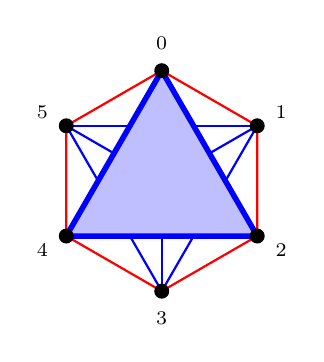
\begin{tikzpicture}[scale=1.0]
    \foreach \i/\ang in {0/90,1/30,2/-30,3/-90,4/-150,5/150} {
        \coordinate (v\i) at (\ang:1.4cm);
    }
    \draw[red, thick] (v0)--(v1)--(v2)--(v3)--(v4)--(v5)--cycle;
    \foreach \i/\j in {0/2,0/3,0/4,1/3,1/4,1/5,2/4,2/5,3/5} {
        \draw[blue, thick] (v\i)--(v\j);
    }
    \fill[blue!25] (v0)--(v2)--(v4)--cycle;
    \draw[blue, line width=2pt] (v0)--(v2)--(v4)--cycle;
    \foreach \i/\ang in {0/90,1/30,2/-30,3/-90,4/-150,5/150} {
        \filldraw[black] (v\i) circle (2.5pt);
        \node[font=\scriptsize] at (\ang:1.75cm) {$\i$};
    }
\end{tikzpicture}\\[3pt]
{\footnotesize Triángulo \textcolor{blue}{0-2-4} monocromático}
\end{center}
\end{columns}
\end{frame}

\begin{frame}{El problema de la amistad}
\begin{columns}
\column{0.50\textwidth}
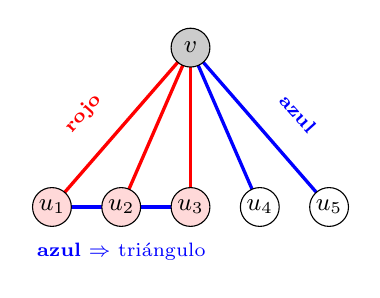
\begin{tikzpicture}[scale=0.88]
    \coordinate (v)  at (0,   2.3);
    \coordinate (u1) at (-2.0, 0);
    \coordinate (u2) at (-1.0, 0);
    \coordinate (u3) at (0,    0);
    \coordinate (u4) at (1.0,  0);
    \coordinate (u5) at (2.0,  0);
    \draw[red, very thick] (v)--(u1);
    \draw[red, very thick] (v)--(u2);
    \draw[red, very thick] (v)--(u3);
    \draw[blue, very thick] (v)--(u4);
    \draw[blue, very thick] (v)--(u5);
    \fill[blue!20] (u1)--(u2)--(u3)--cycle;
    \draw[blue, very thick] (u1)--(u2)--(u3)--cycle;
    \filldraw[gray!40, draw=black] (v)  circle (.28cm);
    \node[font=\small\bfseries] at (v) {$v$};
    \foreach \p/\lbl in {u1/$u_1$, u2/$u_2$, u3/$u_3$} {
        \filldraw[red!15, draw=black] (\p) circle (.28cm);
        \node[font=\small\bfseries] at (\p) {\lbl};
    }
    \foreach \p/\lbl in {u4/$u_4$, u5/$u_5$} {
        \filldraw[white, draw=black] (\p) circle (.28cm);
        \node[font=\small\bfseries] at (\p) {\lbl};
    }
    \node[red,  font=\scriptsize, rotate=48]  at (-1.55, 1.35) {\textbf{rojo}};
    \node[blue, font=\scriptsize, rotate=-48] at (1.55, 1.35)  {\textbf{azul}};
    \node[blue, font=\scriptsize] at (-1.0, -0.65) {\textbf{azul} $\Rightarrow$ triángulo};
\end{tikzpicture}
\column{0.46\textwidth}
    \textbf{Palomar:} $v$ tiene 5 aristas, al menos 3 del mismo color. Supongamos 3 \textcolor{red}{rojas} hacia $u_1, u_2, u_3$.\\[8pt]
    \begin{itemize}
        \item[\textbf{(I)}] Alguna $u_i u_j$ es \textcolor{red}{roja} $\Rightarrow$ triángulo \textcolor{red}{rojo}. $\checkmark$
        \item[\textbf{(II)}] Todas \textcolor{blue}{azules} $\Rightarrow$ triángulo \textcolor{blue}{azul} $u_1 u_2 u_3$. $\checkmark$
    \end{itemize}
    \pause
    \begin{block}{Número de Ramsey}
        $R(3,3) = 6$ es el mínimo $n$ tal que toda 2-coloración de $K_n$ tiene un triángulo monocromático.
        \begin{align*}
            R(3,4)=9 \qquad R(4,4)=18
        \end{align*}
    \end{block}
\end{columns}
\end{frame}
